
%%% Local Variables:
%%% mode: latex
%%% TeX-master: t
%%% End:

% !Mode:: "TeX:UTF-8"

\chapter{基于任务精确预测的实时功耗温度管理}
\label{cha:DPTM}

\section{实时系统的工作负载模型}
\label{sec:workload}
本文讨论的实时系统可以周期性地分配一段时间$D$作为执行某一任务的截止时间,该任务在最坏情况下所需要的执行时间为$W$。 不失一般性,我们假设任务的截止时间等于系统周期性分配的时间片,并且等价地只考虑一个周期内的任务。 文献\onlinecite{RTCalSchHdRTSys}与\onlinecite{LkSchMaxTemMinPerHdRTSys}根据任务的性质研究了如何决定$(D,W)$数据对的值。 本文中,由于可以预测出发送至实时系统的数据量,工作负荷便可以被认为是网络流量的归一化形式。


\section{实时系统的热分析模型}
\label{thermal}
为了研究处理器内核(Die)的热传导特性, 文献\onlinecite{LkDVSRTEmbSys,LkSchMaxTemMinPerHdRTSys,WCTemAnlyRTSys}等都广泛采用了等效RC电路方法进行热分析建模, 并采用如下公式进行工作温度的求解
式中$T$和$T_{amb}$分别代表芯片的温度与环境温度,$P$代表芯片在时刻$t$的功耗,$R_{th}$与$C_{th}$分别为等效热阻与等效热容。


\section{实时系统的功耗分析模型}
\label{power}

处理器的系统状态可以分为工作状态和休眠状态: 只有在工作状态下处理器才执行任务; 否则,处理器将进入休眠状态以减少功耗并降低自身温度。工作状态下的功耗:

式中的第一项代表动态功耗,第二项代表静态功耗。当给定供电电压$V_{dd}$后,工作频率$f$为

由于与工作电压成正比,我们可以得到动态功耗的计算公式

通过HSPICE软件进行的曲线拟合,与温度、电压相关的漏电流可写为

式中$A,B,\alpha,\beta,\gamma,\delta,\mu,\eta$是经验参数,由生产工艺所决定(本文的模拟实验默认选择采用65nm的工艺参数)。 当工作温度$T$在300K到380K的正常范围变化时,$\exp(\frac{1}{T})$的波动变化很小。 当给定了$V_{dd}$后,文献\onlinecite{EngRTTskSchTemDepLk}通过引入两个参考温度$TH$和$TL$进一步将漏电流简化为温度的二次函数。 于是,与漏电流相关的静态功耗可以用下式计算

其中,

此外,处理器的工作状态切换是通过改变工作电压来实现的, 状态切换所带来的开销包括能耗开销$p_r$与延时开销$c_r$\onlinecite{TemIdDistEngOptDVS}。 整体而言,工作状态切换跨度越大,其能耗和时间的开销也就越大。


\section{已有的DPTM调度算法}
\label{algorithms}

\subsection{TALK算法}
TALK及其改进算法\onlinecite{TemLkMinTechRTSys}根据工作负载和截止时间的不同, 来控制不同时间段处理器的工作/休息状态:当负载量大并且温度较低时、处理器处于激活工作状态; 当负载量小并且温度较高时,处理器切换到睡眼状态以减小能耗,以降低温度。


\subsection{Pattern-Based算法(简称PB算法)}

PB算法将任务的截止时间或者运行周期D等分为n个时间片段,每段长$\Delta=D/n$, 采用PB算法的处理器将工作于特定规则的模式中\onlinecite{EngRTTskSchTemDepLk}: 执行$\Delta=D/n$时间后便切入休眠模式,以减少功耗并降低温度。 文献\onlinecite{EngRTTskSchTemDepLk}与\onlinecite{WCTemAnlyRTSys}证明:如果重复这种运行模式足够多次, 处理器将达到温度的平衡值,并进入稳定状态, 即每个周期的初始温度和结束温度将趋向于稳定值,以便于分析。

\subsection{M-Oscillating算法(简称MO算法)}

上面介绍的TALK算法和PB算法都要求处理器的工作速度要大于或者等于负载率$W/D$。 文献\onlinecite{LkSchMaxTemMinPerHdRTSys}证明,如果采用两个最接近的速度完成分配给处理器的任务,那么相对于采用其他的工作速度组合, 处于该速度组下处理器的温度是最优的。 如果进一步地将这种两步策略应用在m个时间片中, 不仅温度可以进一步优化,还可以将D时间内的总功耗表达为m的函数,而且必然存在能耗最小化的$m$值\onlinecite{LkEngMinRTSysMaxTemConst}。 由于要考虑电压切换所付出的时间开销和能耗开销,\onlinecite{LkEngMinRTSysMaxTemConst}给出了m所具有确定的上限值$Ceil$。

\subsection{对已有算法的评估}
作为温敏调度算法,TALK参照剩余任务量与当前温度、来合理地调度任务。 然而,简单的开关模式无法利用DVS技术,只能工作在固定速度。而且状态切换所导致的时间、能耗开销也是不可避免的。 根据切换时间和能耗开销\onlinecite{TemIdDistEngOptDVS},从全速工作转变为零电压将产生最大的能耗和时间开销。
无论采用TALK还是PB算法,都要求处理器工作在大于$W/D$的速度上。 大多数具有DVS或DVFS功能的实时系统通常只允许芯片的电压为若干离散值,根据负载率来调整电压工作档。 这往往会导致芯片实际上工作高于任务所需的速度,不仅增加了近似与电压三次方成正比的动态功耗和与电压近似成正比的静态功耗,而且加速了温度的攀升, 抬高了平衡态时的温度,进一步导致漏电流近似平方速度的增长。
G.Quan等\onlinecite{LkEngMinRTSysMaxTemConst}提出的MO算法存在两个主要缺陷。首先,假设功率为温度的线性函数,使得峰值温度较PB有很大降低。 其次是在实际应用中不能忽略低工作负载率情况:当$W/D$小于处理器支持的最低工作速度时,MO只能退化为PB,以防止不必要的功耗增加。



\section{基于电压预测的TALK算法:VP-TALK}
\label{vp-talk}

\section{DPTM原型系统}
\label{DPTM-system}


\subsection{启发性示例}

\subsection{基于机器学习的DPTM原型系统}

\subsection{基于单一调度策略的DPTM原型系统}







\section{其它例子}
\label{sec:other}

在第~\ref{cha:intro} 章中我们学习了贝叶斯公式~(\ref{equ:chap1:bayes}),这里我们复
习一下:
\begin{equation}
\label{equ:chap2:bayes}
p(y|\mathbf{x}) = \frac{p(\mathbf{x},y)}{p(\mathbf{x})}=
\frac{p(\mathbf{x}|y)p(y)}{p(\mathbf{x})}
\end{equation}

\subsection{绘图}
\label{sec:draw}

本模板不再预先装载任何绘图包(如 \textsf{pstricks,pgf} 等),完全由你自己来决定。
个人觉得 \textsf{pgf} 不错,不依赖于 Postscript。此外还有很多针对 \LaTeX{} 的
 GUI 作图工具,如 XFig(jFig), WinFig, Tpx, Ipe, Dia, Inkscape, LaTeXPiX,
jPicEdt, jaxdraw 等等。

\subsection{插图}
\label{sec:graphs}

强烈推荐《\LaTeXe 插图指南》!关于子图形的使用细节请参看 \textsf{subfig} 的说明文档。

\subsubsection{一个图形}
\label{sec:onefig}
一般图形都是处在浮动环境中。之所以称为浮动是指最终排版效果图形的位置不一定与源文
件中的位置对应\footnote{This is not a bug, but a feature of \LaTeX!},这也是刚使
用 \LaTeX{} 同学可能遇到的问题。如果要强制固定浮动图形的位置,请使用 \textsf{float} 宏包,
它提供了 \texttt{[H]} 参数。比如图~\ref{fig:xfig1}。
\begin{figure}[H] % use float package if you want it here
  \centering
  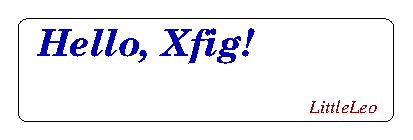
\includegraphics{hello}
  \caption{利用 Xfig 制图}
  \label{fig:xfig1}
\end{figure}

大学之道,在明明德,在亲民,在止于至善。知止而后有定;定而后能静;静而后能安;安
而后能虑;虑而后能得。物有本末,事有终始。知所先后,则近道矣。古之欲明明德于天
下者,先治其国;欲治其国者,先齐其家;欲齐其家者,先修其身;欲修其身者,先正其心;
欲正其心者,先诚其意;欲诚其意者,先致其知;致知在格物。物格而后知至;知至而后
意诚;意诚而后心正;心正而后身 修;身修而后家齐;家齐而后国治;国治而后天下
平。自天子以至于庶人,壹是皆以修身为本。其本乱而未治者 否矣。其所厚者薄,而其所
薄者厚,未之有也!

\hfill \pozhehao《大学》

古之学者必有师。师者,所以传道受业解惑也。人非生而知之者,孰能无惑?惑而不从师,
其为惑也,终不解矣。生乎吾前,其闻道也固先乎吾,吾从而师之;生乎吾後,其闻道也亦
先乎吾,吾从而师之。吾师道也,夫庸知其年之先後生於吾乎!是故无贵无贱无长无少,道
之所存,师之所存也。

嗟乎!师道之不传也久矣,欲人之无惑也难矣。古之圣人,其出人也远矣,犹且从师而问焉;
今之众人,其下圣人也亦远矣,而耻学於师。是故圣益圣,愚益愚。圣人之所以为圣,愚
人之所以为愚,其皆出於此乎?爱其子,择师而教之,於其身也,则耻师焉,惑焉。彼童子
之师,授之书而习其句读者,非吾所谓传其道、解其惑者也。句读之不知,惑之不解,或师
焉,或不焉,小学而大遗,吾未见其明也。巫医、乐师、百工之人不耻相师,  士大夫之族
曰“师”曰“弟子”之云者,则群聚而笑之。问之,则曰:彼与彼年相若也,道相似也,位
卑则足羞,官盛则近谀。呜呼!师道之不复,可知矣。巫医、乐师、百工之人。吾子不齿,
今其智乃反不能及,其可怪也欤!圣人无常师。孔子师郯子、苌子、师襄、老聃。郯子之徒,
其贤不及孔子。孔子曰:“三人行,必有我师。”是故弟子不必不如师,师不必贤於弟子。
闻道有先後,术业有专攻,如是而已。

李氏子蟠,年十七,好古文、六艺,经传皆通习之,不拘於时,学於余。余嘉其能行古
道,作师说以贻之。

\hfill \pozhehao 韩愈(唐)

